%%%%%%%%%%%%%%%%%%%%%%%%%%%%%%%%%%%%%%%%%%%%%%%%%%%%%%%
%
%                                                       Example IS Template
%
% \documentclass{woosterthesis} must be at the beginning of every IS. Options are the same as
% for the report class with some additional options: abstractonly, acs, alltt, apa, blacklinks, chicago,
% code, colophon, dropcaps, euler, foreignlanguage, gauss, index, kaukecopyright, lshortwooster, maple, mla, palatino, picins,tikz,
% verbatim, wblack, and woostercopyright. The kaukecopyright option will put the arch symbol with the word mark on the
% copyright page. The woosterthesis class is based on the report class. One thing to note is that
% the ``%'' symbol comments out all characters that follow it on the line.
%
%%%%%%%%%%%%%%%%%%%%%%%%%%%%%%%%%%%%%%%%%%%%%%%%%%%%%%%

%%%%%%%%%%%%%%%%%%%%%%%%%%%%%%%%%%%%%%%%%%%%%%%%%%%%%%%
%
% Checked on 8/26/22 and compiles with no fatal errors. Users must have the latest version of the TeXLive software and
% have installed all available packages from CTAN to ensure this thesis class compiles with no fatal errors. Also, you must
% run pdfLaTex, Biber, MakeIndex, padfLaTeX, pdfLaTeX to get all the numbering and references resolved. This is the
% first year the template uses Biber for references.
%
%%%%%%%%%%%%%%%%%%%%%%%%%%%%%%%%%%%%%%%%%%%%%%%%%%%%%%%

%%%%%%%%%%%%%%%%%%%%%%%%%%%%%%%%%%%%%%%%%%%%%%%%%%%%%%%
% use this declaration for a draft  version of your IS
\documentclass[palatino,code,picins,tikz,kaukecopyright,openright,lshortwooster,dropcaps,verbatim,index,oneside,euler]{woosterthesis}
% Note that you can specify the acs option to use the American Chemical Society citation format, apa option to use the American
% Psychological Association citation format, chicago option to use the Chicago citation format, mla option to use the Modern Language
% Association citation format, wblack option for a grayscale Wooster "W" on the cover, and scottie option for a grayscale Scottie Mascot
% on the cover. See exampleis_manual.pdf for an explanation of all the options.
%
%%%%%%%%%%%%%%%%%%%%%%%%%%%%%%%%%%%%%%%%%%%%%%%%%%%%%%%
%
% use this declaration for the print version of your IS
%\documentclass[12pt,code,palatino,picins,blacklinks,kaukecopyright,openright,oneside,final]{woosterthesis} % probably what most students would use
%
%%%%%%%%%%%%%%%%%%%%%%%%%%%%%%%%%%%%%%%%%%%%%%%%%%%%%%%
%

% use this declaration for the PDF version of your IS
%\documentclass[12pt,code,palatino,picins,kaukecopyright,openright,oneside,final]{woosterthesis}
%
%%%%%%%%%%%%%%%%%%%%%%%%%%%%%%%%%%%%%%%%%%%%%%%%%%%%%%%

%%%%%%%%%%%%%%%%%%%%%%%%%%%%%%%%%%%%%%%%%%%%%%%%%%%%%%%
%
%                                                       Load Packages
%
%   To load packages in addition to the ones that are loaded by default, please place your
%   usepackage commands in the packages.tex file in the styles folder.
%
%%%%%%%%%%%%%%%%%%%%%%%%%%%%%%%%%%%%%%%%%%%%%%%%%%%%%%%

\input{styles/packages}

%%%%%%%%%%%%%%%%%%%%%%%%%%%%%%%%%%%%%%%%%%%%%%%%%%%%%%%
%
%                                                       Load Personal commands
%                                                                    
%  There will be certain commands that you use frequently in the thesis. You can give these
%  commands new names which are easier for you to remember. You can also combine several
%  commands into a new command of your own. See The LaTeX Companion or Guide to LaTeX
%  for examples on defining your own commands. These are commands that I defined to cut
%  down on typing. You can enter your commands in the personal.tex file in the styles folder.
%
%%%%%%%%%%%%%%%%%%%%%%%%%%%%%%%%%%%%%%%%%%%%%%%%%%%%%%%

\input{styles/personal}

%%%%%%%%%%%%%%%%%%%%%%%%%%%%%%%%%%%%%%%%%%%%%%%%%%%%%%%
%
%                                                       Load Theorem formatting information
%
%  If you need to define an new theorem style or want to see what theorem like environments 
%  are available please look at the theorems.tex file in the styles folder.
%
%%%%%%%%%%%%%%%%%%%%%%%%%%%%%%%%%%%%%%%%%%%%%%%%%%%%%%%

\input{styles/theorems}

\setcounter{secnumdepth}{5}% controls the numbering of sections
\setcounter{tocdepth}{6}% controls the number of levels in the Contents

%%%%%%%%%%%%%%%%%%%%%%%%%%%%%%%%%%%%%%%%%%%%%%%%%%%%%%%
%
%  This is where one enters their bibilography file name.
%
%%%%%%%%%%%%%%%%%%%%%%%%%%%%%%%%%%%%%%%%%%%%%%%%%%%%%%%

\addbibresource{references.bib}

%%%%%%%%%%%%%%%%%%%%%%%%%%%%%%%%%%%%%%%%%%%%%%%%%%%%%%%
%
%  This is where one enters the information about the thesis.
%
%%%%%%%%%%%%%%%%%%%%%%%%%%%%%%%%%%%%%%%%%%%%%%%%%%%%%%%

\title{Investigation of System Architecture, Databases, and Caching systems For backend web development}
\thesistype{Independent Study Thesis} % you should make this Independent Study Thesis
\author{Jungho Park}
% \presentdegrees{Ph.D.} % you should comment this line
\degreetoobtain{Bachelor of Arts}
\presentschool{The College of Wooster}
\academicprogram{MCS}
\gradyear{2026}
\advisor{Drew Guarnera (Computer Science)}
%\secondadvisor{Second Advisor}
%\reader{Reader}
\copyrighted   
%\copyrightdate{}                  
\makeindex % comment this line if you do not have an index

%%%%%%%%%%%%%%%%%%%%%%%%%%%%%%%%%%%%%%%%%%%%%%%%%%%%%%%
%
%  This is where the commands for the document begin. All \LaTeX{} documents must have a
%  \begin{document} text .... \end{document} structure.
%
%%%%%%%%%%%%%%%%%%%%%%%%%%%%%%%%%%%%%%%%%%%%%%%%%%%%%%%

\begin{document}

%%%%%%%%%%%%%%%%%%%%%%%%%%%%%%%%%%%%%%%%%%%%%%%%%%%%%%%
%
%  The front matter includes acknowledgments, dedications, vitas, list of tables, list of figures,
%  copyright, abstract, title page, and contents.
%
%%%%%%%%%%%%%%%%%%%%%%%%%%%%%%%%%%%%%%%%%%%%%%%%%%%%%%%

\frontmatter
\ifthenelse{\boolean{abstractonly}}{
  % Do nothing — skip front matter
}{
\maketitle
\ClearShipoutPicture
\clearpage\thispagestyle{empty}\null\clearpage
\disscopyright 
}

%%%%%%%%%%%%%%%%%%%%%%%%%%%%%%%%%%%%%%%%%%%%%%%%%%%%%%%
%                                                                                       
%                                                       Abstract						
%                                                                                       
%%%%%%%%%%%%%%%%%%%%%%%%%%%%%%%%%%%%%%%%%%%%%%%%%%%%%%%

\begin{abstract}
Include a short summary of your thesis, including any pertinent results.  This section is \emph{not} optional, and the reader should be able to learn the meat of your thesis by reading this (short) section.
\end{abstract}

%%%%%%%%%%%%%%%%%%%%%%%%%%%%%%%%%%%%%%%%%%%%%%%%%%%%%%%
%                                                                                       
%                                                       Dedications					
%                                                                                       
%%%%%%%%%%%%%%%%%%%%%%%%%%%%%%%%%%%%%%%%%%%%%%%%%%%%%%%

\dedication{This work is dedicated to the future generations of Wooster students.}


%%%%%%%%%%%%%%%%%%%%%%%%%%%%%%%%%%%%%%%%%%%%%%%%%%%%%%%
%                                                                                       
%                                                       Acknowledgments					
%                                                                                       
%%%%%%%%%%%%%%%%%%%%%%%%%%%%%%%%%%%%%%%%%%%%%%%%%%%%%%%

\begin{acknowl}  
I would like to acknowledge Prof. Lowell Boone in the Physics Department for his suggestions and code.
\end{acknowl}

%%%%%%%%%%%%%%%%%%%%%%%%%%%%%%%%%%%%%%%%%%%%%%%%%%%%%%%
%                                                                                       
%                                                       Vita					
%                                                                                       
%%%%%%%%%%%%%%%%%%%%%%%%%%%%%%%%%%%%%%%%%%%%%%%%%%%%%%%

\begin{vita} 
% You talk about yourself and how you got to where you are now. There is a structured form for the Vita that can be used if you want, but I don't encourage it.

%%%%%%%%%%%%%%%%%%%%%%%%%%%%%%%%%%%%%%%%%%%%%%%%%%%%%%%
%
%  The list below is for a thesis that requires a more structured Vita such as a masters or Ph.D.
%
%%%%%%%%%%%%%%%%%%%%%%%%%%%%%%%%%%%%%%%%%%%%%%%%%%%%%%%

%\begin{datelist}
%\item[August 11, 1990]Chosen to present an undergraduate paper at the 75th meeting of the MAA, Columbus, Ohio
%\item[August 1990--August 1991]President Wooster Student Chapter of the MAA, The College of Wooster, Wooster, Ohio
%\item[August 1991--May 1992]Secretary Wooster Student Chapter of the MAA, The College of Wooster, Wooster, Ohio
%\item[1992]\emph{Phi Beta Kappa} (on junior standing), The College of Wooster, Wooster, Ohio
%\item[1992]Elizabeth Sidwell Wagner Prize in Mathematics, The College of Wooster
%\item[1992]William H. Wilson Prize in Mathematics, The College of Wooster
%\item[May 11, 1992]B.A., Mathematics, The College of Wooster
%\item[1997]Finalist for Graduate Teaching Award, The Ohio State University, Columbus, Ohio
%\item[June 21-25, 1998]Participant in the AMS-IMS-SIAM Summer Research Conferences: q-Series, Combinatorics, and Computer Algebra, Mt. Holyoke, Massachusetts
%\item[October 1998--October 1999]Graduate student representative to The Ohio State University Department of Mathematics Graduate Studies Committee, Columbus, Ohio
%\item[January 1999]q-series seminar address, The Ohio State University, Columbus, Ohio
%\item[2000]Finalist for Departmental Teaching Award, The Ohio State University, Columbus, Ohio
%\item[2000]Nominated for Graduate Teaching Award, The Ohio State University, Columbus, Ohio
%\item[April 2000]Invited colloquium talk at The College of Wooster, Wooster, Ohio
%\item[1992-- present]Graduate Teaching and Research Associate, The Ohio State University
%\end{datelist}
%
%%%This is for any publications you might have.%%%%%

\begin{publist}  
\pubitem{\quad}
\pubitem{\quad}
\end{publist} 

\begin{fieldsstudy} 
    \majorfield{Major}
	\minorfield{Minor}
    \specialization{Area of IS research}
    %\begin{studieslist}
   %\studyitem{Abstract Algebra}{Hampton}
   %\end{studieslist}
  \end{fieldsstudy}
\end{vita}

%%%%%%%%%%%%%%%%%%%%%%%%%%%%%%%%%%%%%%%%%%%%%%%%%%%%%%%
%
%  We now create the contents page and if necessary the list of figures and list of tables.
%
%%%%%%%%%%%%%%%%%%%%%%%%%%%%%%%%%%%%%%%%%%%%%%%%%%%%%%%


\cleardoublepage
\phantomsection
\addcontentsline{toc}{chapter}{Contents}

\tableofcontents
\listoffigures %Use if you have a list of figures.
\listoftables%Use if you have a list of tables.
\lstlistoflistings% Use if you are using the code option

%%%%%%%%%%%%%%%%%%%%%%%%%%%%%%%%%%%%%%%%%%%%%%%%%%%%%%%


%!TEX root = ../main.tex
\chapter*{Preface}\label{pref}
\addcontentsline{toc}{chapter}{Preface}
\lettrine[lines=2, lhang=0.33, loversize=0.1]{T}he purpose of this document is to provide you with a template for typesetting your IS using \LaTeX\index{LaTeX@\LaTeX}. \lt is very similar to HTML in the sense that it is a markup language. What does this mean? Well, basically it means you need only enter the commands for structuring your IS, i.e., identify chapters, sections, subsections, equations, quotes, etc. You do not need to worry about any of the formatting. The  \texttt{woosterthesis} class takes care of all the formatting.

Here is how I plan on introducing you to \LaTeX. The Introduction gives some reasons for why one might find \lt superior to MS Word\texttrademark. Chapter \ref{text} will demonstrate how one starts typesetting a document and works with text in \LaTeX. Chapter \ref{graphics} discusses the creation of tables and how one puts figures into a thesis. Chapter \ref{bibind} talks about creating a bibliography/references section and an index. There are three Appendices which discuss typesetting mathematics and computer program code. The Afterword will discuss some of the particulars of how a \lt document gets processed and what packages the \texttt{woosterthesis} class uses and are assumed to be available on your system.

Hopefully, this document will be enough to get you started. If you have questions, please refer to \citet{mgbcr04,kd03,ophs03,feu02,fly03}, or \citet{gra96}. % most theses do not have a preface so this should be commented

%%%%%%%%%%%%%%%%%%%%%%%%%%%%%%%%%%%%%%%%%%%%%%%%%%%%%%%
\mainmatter

%%%%%%%%%%%%%%%%%%%%%%%%%%%%%%%%%%%%%%%%%%%%%%%%%%%%%%%
%
%                                                       Thesis Chapters
%
% This is where the main text of the thesis goes. I have written this template assuming that
% each chapter is a separate file. You do not have to do this but it makes things easier to find
% for editing. You can use the sample chapters to help you figure out how to type things into
% your thesis. To include a chapter just use the \include{chaptername} command. Chapters are
% included in the order listed.
%
%%%%%%%%%%%%%%%%%%%%%%%%%%%%%%%%%%%%%%%%%%%%%%%%%%%%%%%

%!TEX root = ../main.tex
\chapter{Introduction}\label{intro}
So why would you want to use \lt instead of Microsoft Word\texttrademark? I can think of several reasons. The main one for this author is that \lt takes care of all the numbering automatically. This means that if you decide to rearrange material in your IS, you do not have to worry about renumbering or references. This makes it very easy to play around with the structure of your thesis. The second reason is that it is ultimately faster than Word\texttrademark. How? Well, after a week or so of using \lt, you will begin to remember the commands that you use frequently and won't have to use the \lt pallet in TeXShop or TeXworks. So, you can just type everything including the mathematics, where with \msw you would have to use the Equation Editor.

I have also tried to make things more efficient by organizing the example folder as follows. There is a \texttt{main.tex} file which is what you will enter all the information about your IS into and is the document you will typeset. \texttt{main.tex} also has explanations about other files that you might need to edit. In addition, there are folders for chapters, appendices, styles, and figures. This structure is there to try and reduce file clutter and to help you stay organized. There should also be a .bib file which you can use as a model for your own .bib file. The .bib file has your bibliographic information.

\lt is easy to learn. For an average IS, the author will only need to learn a handful of commands. For this small bit of effort, you get a tremendous amount of flexibility and a very beautiful document. The following chapters will introduce some of the common things a student might need to do in a thesis.

\section{What is in \texttt{main.tex}?}
Before we move on let's talk a little bit about what is at the beginning of \verb|main.tex|. The file starts with 
\verb|\documentclass{woosterthesis}|, which must be at the beginning of every IS. In the brackets are options for the woosterthesis class. The options are the same as for the \verb|book| class with some additional options 
\verb|abstractonly|\index{woosterthesis options!abstractonly},
\verb|acs|\index{woosterthesis options!acs},
\verb|alltt|\index{woosterthesis options!alltt},
\verb|apa|\index{woosterthesis options!apa},  
\verb|blacklinks|\index{woosterthesis options!blacklinks},
\verb|chicago|\index{woosterthesis options!chicago},
\verb|citeorder|\index{woosterthesis options!citeorder},
\verb|code|\index{woosterthesis options!code},
\verb|colophon|\index{woosterthesis options!colophon},
\verb|dropcaps|\index{woosterthesis options!dropcaps},
\verb|euler|\index{woosterthesis options!euler},
\verb|foreignlanguage|\index{woosterthesis options!foreignlanguage},
\verb|guass|\index{woosterthesis options!guass}, 
\verb|index|\index{woosterthesis options!index},
\verb|kaukecopyright|\index{woosterthesis options!kaukecopyright},
\verb|maple|\index{woosterthesis options!maple},
\verb|minimalstyle|\index{woosterthesis options!minimalstyle},
\verb|mla|\index{woosterthesis options!mla},
\verb|nostyle|\index{woosterthesis options!nostyle},
\verb|palatino|\index{woosterthesis options!palatino},
\verb|picins|\index{woosterthesis options!picins},
\verb|scottie|\index{woosterthesis options!scottie},
\verb|singlespace|\index{woosterthesis options!singlespace},
\verb|tikz|\index{woosterthesis options!tikz},
\verb|verbatim|\index{woosterthesis options!verbatim},
\verb|wblack|\index{woosterthesis options!wblack},
and \verb|woostercopyright|\index{woosterthesis options!woostercopyright}. If no options are specified then the class default options \texttt{letterpaper}, \texttt{12pt}, \texttt{oneside} , \texttt{onecolumn} , \texttt{final}, and \texttt{openany} are used.

The \verb|abstractonly| option will allow you to print just the Abstract. The \verb|acs| option implements the American Chemical Society citation and reference style. The \verb|alltt| option loads the \ip{alltt} package for using typewriter type in various ways and the \verb|apa| option implements the APA citation and reference style. The \verb|blacklinks| option will make the hyperlinks in the PDF version of the thesis black and suitable for printing; normally the links are colored to provide visual clues to the reader. The \verb|chicago| option implements Chicago style citation and references. The \verb|citeorder| option orders the references according to the citation order of the IS. The \verb|code| option will use \ip{listings} style to format program code examples. The \verb|colophon| option will include a colophon which is a section that describes the fonts and other settings used to produce the manuscript. \verb|dropcaps| loads the \ip{lettrine} package for doing dropped capitals and the \verb|euler| and \verb|guass| options load the \ip{woofncychap} package with the named option which will change the look of chapter headings. The \verb|foreignlanguage| option will load the \ip{csquotes} package and either the \ip{polyglossia} or \ip{babel} package depending on if \xt is being used to allow the input and formatting of sections of text in a foreign language. The \verb|index| option will allow the \ip{makeidx} package to be loaded so that if you have index entries they will be added to an index (this reqires additional steps).  The \verb|kaukecopyright| option will put the Kauke Hall symbol with the pre 2021 wordmark on the copyright page.  The \verb|maple| option will load the Maple package for including Maple code. The \verb|minimalstyle| option will use custom styling for the Table of Contents and List of Figures, Tables, and Listings and otherwise revert to the default \verb|book| class styles. The \verb|mla| option implements the MLA citation and reference style. The \verb|nostyle| option will remove all custom styling and revert to the default \verb|book| class styles. The \verb|palatino| option will use the \ip{pxfonts} package which uses the Palatino fonts. The \verb|picins| option will use the \ip{wrapfig} package to allow text to wrap around images and \verb|verbatim| allows one to set verbatim what is entered. The \verb|tikz| option loads the \ip{Ti\emph{k}Z} package enabling users to draw figures in their \lt document. The \verb|singlespace| option will use the \ip{setspace} package to typeset the document in singlespace. The \verb|wblack| option includes an opaque Wooster "W" (as of 8/2021) in the background of the title page instead of the default opaque Kauke Hall image, the \verb|scottie| option includes an opaque grayscale image of the Scottie mascot in the background of the title page instead of the default opaque Kauke Hall image, and the \verb|woostercopyright| option includes a copyright notice with the new (as of 8/2021) Wooster wordmark (see Appendix \ref{options} for images of what these options produce). Adding or deleting options from the comma separated list will change the appearance of the document and some options should only be used after consulting your advisor. Now let's move on to some other things that you'll need to deal with: text, figures, pictures, and tables.
%!TEX root = ../main.tex
\chapter{Theoretical Foundations and Literature Review}\label{text}

\section[Backend Software Design and Architecture Principles]{Backend Software Design and Architecture Principles}\label{sec:newsec}

There are multiple architectural styles that could be applied when designing the backend system of a web application.
The two main categories are monolithic and distributed. Subcategories such as layered services, microservices, event-driven services, are all under 
these two architecture styles. Each of these design have the pros and cons.

\subsection[Monolithic]{Monolithic}
A monolithic application is where all the logical components of the application is deployed as one unit. 
This also means that the application will be run in one process. For example, if there is a stand-alone Python Flask application deployed to a server, 
this is monolithic applications. The general pros and cons of this architecture style are the following:

Pros:
-	Simplicity: Typically, monolithic applications have a single codebase, which makes them easier to develop and understand
-	Cost: Monolithis are cheaper to build and operate because they tend to be simpler and require less infrastructure.
-	Feasibility: Monoliths are simple and relatively cheap, freeing developers to experiment and deliver systems faster.
-	Reliability: Monoliths makes few or no network calls, which usually means more reliable application.
-	Debuggability: If a bug is spotted or get an error stack trace, debugging is easy, since all the code is in one place.
Cons: 
-	Scalability: 
-	Evolvability: Making changes to monolithic applications become harder as it grows. Since the whole application is one codebase, 
  it is not possible to adapt different technology stacks to different domains if needed.
-	Reliability: Since monolithic applications are deployed as a single unit, any bug that degrades the service will affect the whole application.
-	Deployability: Implementing any change will require redeploy8ing the whole application, which could introduce a lot of risk.

\subsubsection[Layered Architecture]{Layered Architecture}

Layered architecture is a sub category of the Monolithic architecture. Applications that are designed with this architecture has three layered parts: 
the presentation layer, the workflow layer, the persistence layer, and the database layer. Each layer has it’s own tasks and separated within one application. 
Presentation Layer:
	The presentation layer is where the UI is displayed and where the users interact with the system.
   All components that are related to the UI will be included in this layer.
Workflow Layer:
	The workflow layer consists all code that are related to logic such as business logic, workflows, and validations. This is where most of the application’s code is contained.
Persistence Layer:
	The persistence layer encapsulates the behavior that is needed to make objects persistent, 
  such as mapping the architecture to code-base hierarchies into set-based relational databases.
Database Layer:
	The database layer is optional. This layer includes the database, or some kind of way to persist information.

Each of the layer may contain multiple problem domains. For example, for a restaurant, there could be domains like place order, 
deliver order, manage recipes, or mange inventory. Different problem domains could exist together in each layer of  the application. 

An implication of the layered monolithic architecture is the MVC design pattern, which is a abbreviation for model view and context.
In MVC, the model represents business logic and entities in the application; the view represents the user interface; 
and the controller handles the workflow, stitching model elements together to provide the application’s functionality, as shown here: (head first software architecture chapter 6)

General Advantages of Layered Architecture:
-	Feasability (Simplicity)
-	Technical Partitioning
-	Data-intensive
-	Performance (if well designed)
-	Quick to build
-	
General Disadvantages of Layered Architecture
-	Deployability
-	Complexity
-	Scalability: Non flexibility in change in problem dodmain
-	Elasticity
-	Testability
Some applications using the layered architecture may have different structure from the original. Some layers might be separated, 
such as the presentation layer being separated from the other layers. Each structure will have advantages and disadvantages within the layered architecture.

\subsubsection[Modular Monolith]{Modular Monolith}
Modular monolith is when an application is divided into different modules within the monolithic system. A module is one domain of the application,
and each domain will have its independent code base. For instance, an application for a restaurant might have different domains such as orders, deliveries, or recipes.
In this case, there could be separate databases for each modules, or multiple schemas within a single database.
It is important to keep in mind that only the code base is independent in the software structure, meaning that since modular monolithics
is still follows the monolithic architecture, the code will be compiled together as a single application and run in one process.
Pros: 
-	Domain partitioning: each domain will be implemented in a different module, which allows to build teams that specializes in one or more of these domains.
-	Performance: Since there are no network calls within the application like other monolithic applications, performance is good.
-	Maintainability: Each module are separate from each other.
-	Testability:
Cons:
-	Hard to reuse: Since each module have its own code, it is hard to reuse the logic and utilities across the modules
-	Single set of architecture: Since all the code is within one application, logics and databases could become complicated, making it hard to scale.

\subsubsection[Microkernal Architecture]{Microkernal Architecture}
The microkernel architecture is consisted with a core of the application, and plugins. 
The core of the application is where the main application is being run, and the plugins are connected to the core application. 
It is used when a lot of customization is needed for the software
\subsection[Distributed Systems]{Distributed Systems}\label{sec:newsec}
Distributed architecture is when the logical componnents of the application are split up into multiple units. 
These units each run in their individual process and communicate with each other over the network. 
This architecture style encourage loose coupling of each services. The general pros and cons of this architecture style are the following:

Pros:
-	Scalability: Distributed architectures deploy different logical components separately from one another, so it is easy to add new services.
-	Modularity: Distributed architecture encourage a high degree of modularity because their logical components must be loosely coupled.
-	Testablility: Each deployment only serves a select group of logical components. This makes testing a log easier-even as the application grows.
-	Deployability: Distributed architectures encourage lots of small units. They evolved after modern engineering principles like continuous integration, 
  continuous deployments, and automated testing became the norm.
-	Fault Tolerance: Even if one piece of the system fails, the rest of the system can continue functioning.
Cons:
-	Performance: Distributed architectures involve lots of small services that communicate with each other over the network.
  This can affect performance, but there are ways to improve this.
-	Cost: More servers are needed to deploy multiple units. These services will need to talk to each other, which entails setting up and maintaining network infrastructure.
-	Simplicity: Distributed systems are complicated to understand from how they work to debugging errors.
-	Debuggability: Errors could happen in any unit involved in servicing a request. Since logical components are deployed in separate units,
  tracing errors could become complicated.

There are both advantages and disadvantages for monolithic and distributed systems and choosing the appropriate architecture for each situation is crucial.
After deciding which of the two main architecture will be used, then we could decide on which subcategory of either of the architecture to implement.
Same as the monolithic structure, distributed systems architecture has multiple types of subcategories, each having advantages and disadvantages. 

\subsubsection[Microservices Architecture]{Microservices Architecture}

A microservice is a service that is separately deployed unit of software that performs some business or infrastructure process.(chapter 10).
A microservices architecture is part of the layered system, where microservices communicate which each other to make an application. 
Since the system is divided into multiple parts, it is essential how to divide the application, 
such as deciding how small or how big each microservices could get into. Generally, it is better to make microservices smaller for 
multiple reasons. Some of the factors that is considered to make microservices 
smaller are the following: cohesiveness, fault tolerance, access control, code volatility, and scalability. 

If a part of the software has lack of cohesiveness and loosely coupled, it is a good idea to separate it into smaller microservices. 
This will allow higher scalability. If a certain part of the application produces fatal errors, 
having those part in a sparate microservice will decrease the probability to shut down the whole system. 
For security and authentication, it is important to have these access controlabilities into a single microservice, 
so it does not get too complicated when managing the information. Finally, if one part of the microservice change, 
or scale faster than the others, it is good to consider to have a separate microservice for that application, 
since testing the entire microservice would be much more challenging compared to a small portion of the microservice. 

On the other hand, there are times when it is encouraged to make the microservices bigger: Database transactions, data dependencies, and workflow. 
It is not possible to perform a single database commit or rollback when a request involves multiple microservices. 
For data consistency and integrity, it is important to combine functionalities that require these kind of behavior into a single microservice. 
If a part of a microservice has highly coupled data, such as when a database table refers to  the key of another database table, 
it is better to keep these functionalities as a single microservice, to keep the data integrity of the database. 
If a single request requires separate microservices to communicate with each other, this request is coupled. 
If too much coupling is occurred between microsesrvices, there are many negative effects. 
For example, performance is affected by network, security, and data latency. 
Scalability is affected because each microservice in the call chain must scale as the other microservices scale (something that is hard to coordinate).
Fault tolerance is affected because if one of the microservices in the chain becomes unresponsive or unavailable, the request cannot be processed.
It is good practice to consider the workflow and decide whether to keep the microservice big.\\

\noindent \textbf{Balance}

\noindent Sharing functionalities

There are many times when the same code has to be used in multiple microservices. 
There are mainly two ways for sharing code when building a microservice architecture. 
Creating a shared service, or a shared library.  
A shared service is a separate microservice that contains a shared functionality that other microservices can call remotely.
The advantages of using this is that eventhough a code is changed in the shared microservices, code in other microservices are not required to change.
Also, this shared service could be written in any language, which is useful when microservices are implemented in multiple languages. 
A disadvantage of using a shared service is coupling that happens between the microservices and the shared service. 
This leads to risks when changing a shared service since it can affect the other microservices that call it.
Furthermore, when the shared service is down for some reason, the microservices that require the shared service would not function.
Another disadvantage is network latency, ….

A shared library is a more common way for code reuse. A library will be built including all the code that are reused in different microsesrvices,
and once they microservices are deployed, each microservice will have all the shared functionality available. 
The biggest advantage of using a shared library is that network performance and scalability is better than shared service, 
since it is not remote and the code is included in the compile time of the microservice. 
However, multiple shared libraries will be needed if microservices are written in different programming languages. 
Also, managing dependencies between microservices and shared libraries could be a challenge if there are multiple microservices using the shared code. \\


\noindent \textbf{Workflow}

Microservices communicate with each other to make the whole application. It is important to know how these are connected, 
and this is where workflow comes in.
The term workflow means when two or more microservices are called for a single request. 
Workflows are in charge of navigating which microservice to start, which one to call next, and which one to end with.
There are two ways to handle workflows: centralized workflow management, and decentralized workflow management. 

\noindent \textbf{Centralized workflow management}

This workflow management style is where there is a microservice that coordinates all the microservices that are needed to handle a 
certain single request. This microservice will be responsible for calling all related microservices, knowing the current state of the 
workflow and what happens next, summarize all data from each microservice, and handling errors. 

The advantage of this workflow management style is that the order of microservices for each requests are clear. The central microservice always has the exact routes the request hast to take, which allows to track the status where each requests stopped and where to restart. This allows to handle errors efficiently. Also, it is easy to change a workflow since this all changes in one central microservice.

The disadvantage is that tight coupling between the central microservice and the other microservices. This can lead to lower scalability, since changing a microservice will affect the central microservice. Moreover, performance might get delayed since the central microservice is indeed another microservice that requires remote calls and it saves the workflow state data in a database which slows down the performance. 

\noindent \textbf{Decentralized workflow management}	

The decentralized workflow does not have a central microservice, but rather all microservices redirect to another microservice 
by the given request until the request is complete. It is important to not use one of the microservices as a central microservice.

The advantage of using this workflow pattern is that it is loosely coupled compared to the central workflow management, 
which has better scalability. Also, since the microservices does not have to connect back to the central microservice, 
it has better responsiveness, meaning less delay and better performance. 

On the other hand, this pattern lacks in error handling, since each microservice is responsible for managing the error workflow, 
which could lead to too much communication between services. Also, because there is not a central microservice that has the order 
of microservices that needs to be called, it is hard to tell which state the response is at, which decreases the ability to recover 
when the request is delayed and needs to be restarted again. 

\noindent \textbf{Pros and Cons of microservice architecture.}

Microservice architectures are commonly used and it is important when choosing this software architecture. 
There are multiple advantages when choosing to implement the microservice architecture. 
Loose coupling is a huge advantage. Since each microservices are single-purpose and they are deployed separately, 
and easy to maintain. This means that it is easy to change a particular function that needs modification. 
Also, it is easy to test the application, as the scope is much smaller compared to the monolithic architecture. 
Fault tolerance is another advantage that comes from loose coupling. Even if a particular microservice fails, 
it does not break the whole system. Furthermore, microservice architecture is easy to scale and evolve since we just have to add or 
modify a microservice related to the area. 

However, there are also disadvantages of using the microservice architecture. 
This architecture is complex. It requires multiple decisions(the aspects discussed above: workflow, shared code etc..) 
depending on the situation. Since it is complex, as microservices communicate with each other, the performance also decreases.
The request might have to wait for the network or undergo additional security checks and make extra database calls.
Lastly, deploying all of these microservices will increase the cost of the entire application.  

\subsubsection[Event-Driven Architecture(EDA)]{Event-Driven Architecture(EDA)}
\noindent \textbf{What is an Event}

An event in computer science is a way for a service to let the rest of the system know that something important has just happened. In EDA, events are the means of passing information to other services (head first chapter11). The event contains data and it is broadcasted to services using topics that are connected to the sender of the event. However, events are asynchronous, which means that although the services are connected, the sender of the event does not wait on the response of the receiving service. This is the key difference between a event and message. Messages includes a command or some kind of a request for the receiving service, and the service sending out the messages require a response, making it synchronous. Messages are also sent to only a single service using queues. 

\noindent \textbf{Asynchronous vs Synchronous}

Asynchronous communications do not need to wait for the response, even though the receiving services are available or not. These kinds of communications are also called Fire and Forget. On the other hand, synchronous communication needs to stop and wait until the response, which means that the service in response must be available. EDA relies on the asynchronous communication when sending and receiving events.

\noindent \textbf{Advantages, Disadvantages of Asynchronous Communications}

Asynchronous communications has advantages in responsiveness compared to synchronous communications. Since responses by the receiving services are unnecessary, it takes less time to complete a request. However, this is also a crucial disadvantage. Since we do not know if the receiving services have successfully completed the request, it is prone to error handling. Here is a diagram. 

\noindent \textbf{Advantages of EDA}

Event Driven Architecture is highly decoupled, which makes all services independent and easy to maintain. Furthermore, the asynchronous communication increases the performance of the application. Since EDAs are highly decoupled with this type of communication, it is easy to scale and evolve. 
Disadvantages of EDA
Similar to microservices, EDAs are complex. Deciding which database topology for the architecture, asynchronous communications and parallel event processing makes adds complexity to the application. Also, asynchronous communication makes it more difficult to test out the program. Since the request is proceeded without any response or synchronous calls, the context of the test is vague. If the application needs multiple synchronous calls, EDA is not the right choice for the product. 




\section[Databases]{Databases}\label{sec:newsec}

\subsection[Types of Databases]{Types of Databases}
There are mainly two types of database that are used in software engineering: Relational database and non-relational databases. 
These two databases defer by how they store and data, which influences different aspects if databases including the structure, data integrity mechanism, performance and more. 

\subsubsection[Relational Databases]{Relational Databases}
Relational Databases store data in tables by columns and rows, where each column represents a specific data attribute, 
and each row represents an instance of that data(aws document). Each table must have a primary key, which is an identifier column that identifies the table uniquely.
The primary keys are used to establish relationships between tables, by using the related rows between tables as the foreign key in another table. 
Once two tables are connected, it is now possible to get data from both tables in a single SQL query.

\noindent \textbf{Advantages and Disadvantages}

Relational databases follow a strict structure, which allows users to process complex queries on structured data while maintaining data integrity and consistency. 
The strict structure also follows the ACID (atomic, consistency, isolation, and durability) properties for enhanced data integrity. 
However, because of the rigid structure, it is hard to scale compared to nonrelational database.  

\subsubsection[Non-Relational Databases]{Non-Relational Databases}
Nonrelational databases means that there isn’t a schema to manage and store data. 
This means that data does not require constraints that the relational database required, such as fixed schema, primary key constraint, or not null constraints. 
This allows more flexibility in the structure and size of the database, or anything that may change in the future. 
There are different types of non relational databases: Key-Value databases, Document database, and Graph database. 
Key-Value database store data as a collection of key-value pair, where the key is served as the unique identifier. 
Both the key and values could be anything as objects or complex compound objects. Document databases are used to store data as JSON objects. 
Since it is readable by both human and the machine, it has the ease of development. Lastly, there are graph databases, 
where they are used when a graph-like relationships are needed. Unlike the relational databases, which store data in rigid schema, 
graph databases store data as a network of entities and relationships, providing more flexibility to anything that is prone to change. 

\noindent \textbf{Advantages and Disadvantages}

Nonrelational databases have a less rigid structure allowing more flexibility.
This is useful when the data changes requirements often. For example, when a specific table needs to changes in columns, 
this would be hard to preform because other tables might be associated with the specific column. 
However, nonrelational databases are not constraint to fixed schema, which allows easy changes on specific columns or unique identifier.
Performance is another strength of nonrelational database. 
The performance of these databases depend on outer factor such as network latency, hardware cluster size,
which is different from relational databases which depends internal factors such as the structure of the schema. 
However, because of the flexibility in the structure, data integrity is not always maintained. 
Consistency is an issue since the state of the database changes over time as structures might not be consistent.




\subsection{Database Design and Evolution}
The design of databases and quering the database are the ones that has the most impact on the performance of the database.
In this subsection, we will be talking about ways to structure and queyr efficient database systems.

\subsubsection[Normalization]{Normalization}
Compared to a nonrelational database, relational databases benefit from integrity, with the process of normalization. 
The definition of normalization is a way of organizing data in a database. 
During this process, redundant data will be reduced to improve data quality and optimize database performance. 
There are types of normalization such as 1NF and 2NF, and as the normal form gets higher, 
it is a better design of the relation. However, most databases tend to be needed until the third normal form, 
which avoids most of the problems common to bad relational designs. 

\textbf{The Second Normal Form(2NF)}
The two criterias that 1NF meet are the following:

\begin{enumerate}
    \item The data are stored in a two-dimensional table.
    \item There are no repeating groups. (rddI chapt 7)
\end{enumerate}


Here the repeating groups mean that if an attribute that has more than one value in each row of a table. (relational database design and implementation 4th) 
For instance, if there is a column that requires more than one value, such as items (instead of item), this will be a repeating group. (show table) 
Having three or more dimensions or having repeated groups for a single table results in more complexity and difficulties when querying the database. 
This is why we need the 1NF normalization.The 1NF is the most simple normalization that could be done in a relational database and it is pretty clear. 
However, the first normalization form is not enough from benefiting from using relational databases. 

\textbf{Problems with 1NF}

Data could become redundant even though repeated rows are deleted. 
For example, If there is a table called students with columns(id, name, birthday, course id, course name), every time the same student adds a class, 
their name will be repeated in each record. Furthermore, there are anomalies in update, insertion, and deletion. 
Making an update to one of the records (student name) 
would require to update other records that are associated. Missing out any of the records with the student name will result in data inconsistency. 
Inserting a new entity could be difficult unless there are related data. For instance, if a new course is to be added to the table, 
this would be unavailable until there is a student taking the course since the primary key will be the student’s id, and there could not be a row without a primary key. 
Deletion could also be a problem when the row deleted contained the last data for a certain column. For example, 
if one student is taking a class called CS200, and that record is deleted, the table would not have the information that the class CS200 exists. 
To solve these problems, we must use higher levels of the normalization form.

\textbf{The Second Normal Form(2NF)}

The two criterias that 2NF meet are the following:
\begin{enumerate}
    \item The relation is in first normal form
    \item All nonkey attributes are functionally dependent on the entire primary key. 
\end{enumerate}

Functional dependency is the key term in the 2NF. A functional dependency is a one-way relationship between two attributes, 
such that at any given time, for each unique value of attribute A, only one value of attribute B is associated with it throughout the relation (RDDI chapt7). 
In other words, this means that all other columns except the columns of the primary key or keys, are dependent on the primary key or the candidate key. 

By using the functional dependencies, we could create the second normal form relations. After analyzing the functional dependencies, 
primary keys would be decided. It is common to decide attributes that have dependencies 
for the primary key of the table, and the all the other attributes will be the non-key attributes. 
For example, going back to the student table example, Student name, and birthday would be dependent on the student id, so the student id will be the primary key. 
Courses the student takes does not depend on the student id, but rather on the course id. 
We could create another table using the course id as the primary key, and the course name as the functional dependencies. 
However, the courses the student takes will be dependent on the courses, so there will be a foreign key to construct that relationship. 
So far, we can identify the relationship of the tables as the following:

So far, we can identify the relationship of the tables as the following:

\begin{itemize}
    \item \textbf{Student}(\textit{student\_id} (PK), \textit{course\_id} (FK), \textit{name}, \textit{birthday}, \textit{room\_num}) 
    \item \textbf{Courses}(\textit{course\_id} (PK), \textit{name})
\end{itemize}

\noindent
*We are assuming that each student can only take one course.*

\noindent
The relationship can be represented as:
\[
\text{Student}(\text{course\_id}) \rightarrow \text{Courses}(\text{course\_id})
\]

By doing this, some of the problems from the first normal form are solved. 
The functional dependency solves the insertion, deletion, and update anomalies.
We can now insert a new course into the course table without needing to insert a student at the same time, 
delete a student’s course without losing the record of the course itself, and update course information in one place instead of multiple rows, 
which preserves data integrity. This will provide more stable and consistent database design compared to 1NF.

\textbf{Problems with 2NF}

Although some of the problems with 1NF were solved, there are still anomalies to be resolved. Insertion, deletion, and update anomalies still exist. For example, let us assume we have the following dependencies:

\begin{itemize}
    \item \textbf{Student}(\textit{student\_id} (PK), \textit{course\_id} (FK), \textit{name}, \textit{birthday}, \textit{room\_num}) 
    \[
    \text{Student}(\text{course\_id}) \rightarrow \text{Course}(\text{course\_id}, \text{name}, \text{room\_num} (FK))
    \]
    
    \item \textbf{Course}(\textit{course\_id} (PK), \textit{name}, \textit{room\_num} (FK)) 
    \[
    \text{Course}(\text{room\_num}) \rightarrow \text{Room Number}(\text{room\_num} (PK), \text{name})
    \]
    
    \item \textbf{Room Number}(\textit{room\_num} (PK), \textit{name})
\end{itemize}

Even though the tables are in 2NF, insertion, deletion, and update anomalies can still occur due to these transitive dependencies.

The functional dependency Course -> Room Number introduces anomalies that still remain in 2NF. 
For example, we cannot record a student’s enrollment in a course if the course’s room number has not been decided, which creates an insertion anomaly. 
Also, if we delete the last student enrolled in a course, we also lose the record of the room number for that course, which is a deletion anomaly. 
Finally, if a course’s room number changes, we must update it in every student’s record for that course, creating an update anomaly. 
These problems occur because the room number depends on the course (a non-key attribute) rather than directly on the student ID, 
and they are resolved by moving the design into 3NF.

\textbf{The Third Normalization Form(3NF)}
The two criterias that 3NF meet are the following:

\begin{enumerate}
    \item The relationship is in second normal form.
    \item There are no transitive dependencies.
\end{enumerate}

\textbf{Transitive dependencies}
Transitive dependencies exist when the following functional dependency pattern occurs:  
\[
A \rightarrow B \text{ and } B \rightarrow C \text{, therefore } A \rightarrow C
\] 
(Chapter 7).  

This is the same type of relationship where we had problems with 2NF. For example:

\begin{itemize}
    \item \textbf{Student}(\textit{student\_id} (PK), \textit{course\_id} (FK), \textit{name}, \textit{birthday}, \textit{room\_num}) 
    \[
    \text{Student}(\text{course\_id}) \rightarrow \text{Course}(\text{course\_id}, \text{name}, \text{room\_num} (FK))
    \]
    
    \item \textbf{Course}(\textit{course\_id} (PK), \textit{name}, \textit{room\_num} (FK)) 
    \[
    \text{Course}(\text{room\_num}) \rightarrow \text{Room Number}(\text{room\_num} (PK), \text{name})
    \]
\end{itemize}

Going back to this example, we can see that a non-key attribute in the \textbf{Student} table (\textit{room\_num}) depends on another non-key attribute (\textit{course\_id}).  

To remove transitive dependencies, we should break the relations into separate tables. In this case, we can:

\begin{itemize}
    \item Remove the \textit{room\_num} column from the \textbf{Student} table to remove the relationship between non-key attributes.
    \item Alternatively, make the second determinant in a table a candidate key so that no non-key attribute depends on another non-key attribute within the same table.
\end{itemize}

Applying either method will resolve the anomalies we encountered in the second normalization form (2NF).




\subsubsection[Database Evolution]{Database Evolution}

The database design also has influence on how the database evolves over time. As the size of data increases, performance, latency, and fault tolerance are affected by the database designs. There are multiple techniques to design a database suitable for scaling. Vertical scaling refers to when the physical parts of the computer such as CPU or RAM is upgraded so that the database could handle more data and queries. Horizontal scaling is when having multiple machines with independent physical parts (CPU and RAM), but stores the data on an array of disks that are shared among multiple other machines. 
One advantage of using vertical scaling is that the structure is very simple. Only one database needs to be taken care of, which could be easier compared to handling multiple databases. However, there are more disadvantages. Cost increase faster than linearly as higher performance is required. Fault tolerance is another thing as there is only one database running, failure in the service will damage the connected services. 
For horizontal scaling, there are mainly two strategies that we will discuss: replication and partitioning. These two strategies have its own sub strategies which will be discussed in the next subsection.

\paragraph{Replication:}

The definition of replication is when there are multiple copies of the database in different locations. This leads to redunduntcy in data, but it also allows fault tolerance in case a database is unavailable. (Designing Data Intensive ch5) Some other reasons why someone might want to use a replica is to increase availability by having databases in different regions to decrease latency. Also, having multiple database to read queries also help increase the performance of the application. 

There are multiple ways to implement this strategy in different situations. The three topics discussed will be Leader and Followers, Multi Leader Replication, and Leaderless Replication.

\paragraph{Leaders and Followers:}
Going deeper into how the replicas are actually set up, it is important to make sure that each of the replicas have the same data. For example when a user updates a table, this should include all the other replicas to update the same table. The leader and follower structure has one lead node(leader) that allows writes to the database, and the rest of the nodes are assigned as followers. If there is a change data in the leader, the followers are updated accordingly. Reading the database could be done by any of the nodes including the leader node, but writing the database could only be done by through the leader node. Here is a quick example how the flow might look like
(add an example figure)

\subparagraph{Synchronous vs Asynchronous Replication}
One important factor when setting up replication of databases are whether the replication happens synchronously verses asynchronously. After the leader receives a write query, synchronous replication waits until all of the followers are updated and synced. The leader will not take any queries before this process is finished. However, asynchronous replication keeps taking queries regardless of the status of the followers. Although database replications are fast which usually happens less than a second(Designing Data-Intensive Applications ch 5), there is no guarantee of how long it would take to perform a synchronous replication. This is an advantage of synchronous replication, since it is certain that all database replications are up-to-date with the leader database, but it could be a disadvantage in a perspective where the database queries will be slow. If all of the followers are synchronous, the system would be too slow. Most of the times, one of the followers will be set to being synchrounous so that there will be at least two replications(one leader, one follower) up-to-date with all the write queries, and the rest of the followers being asynchronous. This configuration is sometimes also called semi-synchronous. (Designing Data-Intensive App ch5) 

Asynchronous replications on the other hand are very fast since the leader does not have to wait until the followers are have synced data. However it does have a disadvantage that all of the followers might not be up-to-date right away, which is also known as the replication lag. This might sound like a huge disadvantage, but asynchronous replication is often times used if there are many followers or if they are geographically distributed. Eventually, all the followers will have a synced replication of the leader, since inconsistency is just a temporary state. This effect is called as eventual consistency (Designing Data-Intensive App ch5). If the application that is being created is okay with possibility of inconsistency due to replication lag, asynchrounous replication is perfect. However, if consistency is crucial to the application, other solutions such as synchrounous or semi-synchronous replication will be the go-to when using leaders and followers method. 


\paragraph{Multi-Leader Replication}
One down side of a Leader and Follower replication was that the write queries were only allowed in the leader replica. If the application could not connect to the leader for any reason such as network causes, write queries could not be performed. Multi-Leader replication allows multiple leaders, which means that write queries could be done in multiple replicas. 
Although it is rare for a multi-leader replication structure to over weigh the benefits among the complexity added, there are a few use cases for this structure.
\begin{itemize}
    \item Multi datacenter operation
    \item Clients with offline operation
    \item Collaborative editing
\end{itemize}
However the biggest issue in the multi-leader replication structure is handling multiple write query conflict. This was not an issue for a single leader and followers structure since only one leader accepted write queries and they were processed one by one. However, if multiple leaders receive queries at the same time, the conflict should be resolved. There are multiple ways to handle write conflicts.

The simplest strategy is to just avoid the conflicts. If the write queries could be avoided in the application layer, where the application ensures that all write queries for a particular record go through the same leader. This would work until a particular records needs to change its designated leader. In this case, simply avoiding conflicts in the application layer would not work

The next strategy is to converge toward a consistent state. When there is a situation where avoiding conflicts do not work, the conflicts should be handled. There are various ways to converge the replicas into a consistent state. One way could be to simply give each write query a unique ID, and if there is a conflict, the higher unique ID overwrites the conflict. Another way is to give each replica a unique ID, and the higher unique ID overwrites the conflict. Or, there could be another explicit data structure that preserves the information and write application code to resolve the conflict in a certain logic. There are trade offs such as which part of the data is going to be saved over the other, so it is essential to choose the write way to handle write conflicts in a multi-leader replica structure.

Replication is a way to not only have fault tolerance but also improve the performance of the database. This will be useful as the size of the database and the application grows. It is essential to choose the right strategy for replication depending on the situation to support the evolution of databases and maximize performance.

\paragraph{Partitioning:}
Partitioning is when a data is divided into multiple smaller pieces of data such as a record, a row, or a document. Replication was used for scalability and performance, but as the size of the database increases, only replication itself become inefficient since all the data has to be copied to the replicas. In order to scale database applications, partitioning is commonly used. As the data is distributed among multiple partitions, multiple queries could be ran at the same time. 

\subparagraph{Partitioning by Key-Value Data}
Having a key-value data is one way to create partitions. The reason for partitioning was to scale the database by distributing the query load on one node. One way to achieve this is to have a key range for each partition. For example, when we think of a dictionary, we know that words that start with the letter “a” is in the beginning, the letter “m” is somewhere in the middle, and the letter “z” is at the end. By dividing the range of partitions by the key-value data, it will be easier to locate which partition contains the data and distribute the query. In this case, the partitions might not be evenly divided since the each range of key-value pairs could contain a different amount of data. It is important which key-value pair to use. If a key is assigned as a column that is not evenly distributed, this leads to a hot spot (a partition with disproportionately high load) (Designing Data-Intensive App  ch6). 

A method that has a lower chance of being affected by hot spots is partitioning by hash of key. A good hash function makes a the key-value pairs evenly distributed among the partitions. However, this looses the efficiency that the key range had. It is now hard to find the range queries efficiently without the key range. 

When choosing the strategy, hashing keys and having key ranges to partition data both have advantages and trade-offs, so it is important to choose the one suitable in the situation. Key range could be used if there is a key range that is evenly distributed, and key hash when there are still a lot of hotspots by using the key range. 

\subparagraph{Partitioning and Secondary Indexes}
Partitioning by key-value pairs work nicely with the partitioning strategies discussed above. However things get more complicated with secondary indexes. Secondary indexes will be discussed more in the upcoming sections. A brief introduction for secondary indexes is that they are created to improve the query performance that are based on multiple keys. For example, when searching for a job in a job board, selecting criteria such as industry or experience level could be a situation to use secondary indexes. Secondary indexes makes sharding more complicated since they don’t identify a single record, but rather search for records based on the conditions. Partitioning by key-value pairs wouldn’t work in this situation.

Scatter/gather is a technique where each partition has its own secondary indexes. In this case, writing data would be efficient since only the partition containing that specific part of the index is where the data is written. However, reading queries are less efficient.  If queries require to search on different partitions, each partition is searched separately which is inefficient. 

It is also possible to partition secondary indexes by the term. Instead of having distributed secondary indexes across the partitions, this approach has a global index that covers all the partitions. Having a range of secondary indexes partitioned in separate partitions make read queries more efficient from the scatter/gather technique. If write queries are used more often, it is better to use the scatter/gather technique, and if read queries are dominantly used, partitioning indexes by term is the structure to choose. 

\paragraph{Request Routing}
After partitioning the dataset into multiple nodes, it is important to make sure the request connects to the right partition. On a high level there are mainly three ways to achieve this. 
\begin{enumerate}
    \item Allow clients to contact any node (e.g., via a round-robin load balancer). If that node coincidentally owns the partition to which the request applies, it can handle the request directly; otherwise, it forwards the request to the appropriate node, receives the reply, and passes the reply along to the client.
    \item Send all requests from clients to a routing tier first, which determines the node that should handle each request and forwards it accordingly. This routing tier does not itself handle any requests; it only acts as a partition-aware load balancer.
    \item Require that clients be aware of the partitioning and the assignment of partitions to nodes. In this case, a client can connect directly to the appropriate node, without any intermediary. (Designing Data-Intensive App Ch 6)
\end{enumerate}

The key problem is that how does the component, (which could be the routing tier, the client, or the partition in the node) know about changes in the other partitions in other nodes? If the deciding component is not up to date with the location where data that the client is requesting, this could lead into data inconsistency. 

To solve this problem, many distributed data systems use a separate coordination service such as the ZooKeeper to keep track of the data. The whenever a partition changes or a node is added or removed the ZooKeeper is updated to keep data consistency. 

\paragraph{Performance and Querying Optimization}
There are multiple factors that affect the performance of the database. The design of the database, including normalization, and partitioning, which was discussed in the previous subsection is one of the factors. Indexing is another huge part of increasing the performance of the database as the amount of data increases. Lastly, changing the physical query of the database is a way optimize the performance of the database. In this section, we will be discussing about specific ways to optimize performance of databases.

\subparagraph{Indexing:}
Suppose that there is a table called students with the following keys: id, name, grade. If we want to find students with a certain grade (80\%), we could run a SQL query something like this.
\begin{verbatim}
SELECT * 
FROM Students
WHERE grade = 80;
\end{verbatim}
This query will visit all the rows and then find the students with grades 80. However this query becomes more inefficient as the size of the table grows, as the time complexity would be O(n). If the table was sorted by grades, this will be much easier, since we could do a binary search to make the search speed O(log n). This is where indexing is applied. 

An index could be created where the grades are sorted in order, each having a reference to the row of the student table. This way, whenever we want to find the name of the students with a certain grade, instead of looking at the Students table, we can look at the index, where the grades are sorted, find rows with the certain grade, for each row find the reference of the student table, and return the name of the student. This shows that Indexes significantly improves the read queries for databases. 

There are multiple data structures that could be used to implement indexes, but the most common one are b+trees. B trees are somewhat similar to the binary search trees. However, instead of having one value every node, it contains multiple nodes. This allows multiple partitions, allowing a balanced, and a faster search. Furthermore, as multiple values could be in a single node, the height of the tree would be smaller. This means that there are fewer disk I/O’s per file operation as database stores data on disk, resulting in faster query execution(pg 645 Database Systems the Complete Book). One down side of b trees is when making range queries, such as finding all students who have grads 20 to 80. If these two data are separated from the root, this could be inefficient. (create diagram). B+trees are a variation of b trees to solve this issue. B+trees store data only in the leaf node. The other nodes store keys only for navigation. Also, all the leaf nodes are connected to the next leaf node. (create diagram and explain). 

B+trees are commonly used in indexes for modern databases management system such as MYSQL, PostgreSQL, and SQLite. 

\subparagraph{Query Optimization:}
Optimizing the SQL queries could also increase the performance of the database. Here are the 6 queries tune SQL queries. 
\url{https://www.geeksforgeeks.org/sql/sql-performance-tuning/}
\begin{itemize}
    \item SELECT fields instead of using SELECT *
    \item Avoid SELECT DISTINCT
    \item Use INNER JOIN instead of WHERE for Joins
    \item Use WHERE instead of HAVING
    \item Limit Wildcards to the end of a search term
    \item Use LIMIT for sampling query results
\end{itemize}

\paragraph{N+1 problem}
The N+1 problem is a common problem when using the ORM. The definition of the problem is when an application retrieves a list then performs additional queries for each item’s related data, which results in an inefficient query. (1 + N queries instead of optimized joins). In a nutshell, it is just having too much queries that decreases the performance. This problem usually happens in ORMs. 

Similar to the example above, assume there is a students table with keys student\_id, student\_name, and another table called courses with the keys course\_id, student\_id, and course\_name. 

If we were to get all students and courses they are taking in plain SQL, we would write something like this:
\begin{verbatim}
SELECT s.student_id, s.student_name, c.course_name
FROM students s
JOIN courses c ON s.student_id = c.student_id;
\end{verbatim}



\section[Caching]{Caching}\label{sec:newsec}

\subsection[Client Side Caching]{Client Side Caching}
CDN
HTTP Caching
\subsection[Client Side Caching]{Client Side Caching}
Redis

%!TEX root = ../main.tex
\chapter{Working with figures and tables}\label{graphics}

\section{Getting a simple figure in the document}
In this chapter we want to talk about including figures and tables in the document. To insert a simple figure, you can enter something like
\begin{singlespace}\small
\begin{verbatim}
\begin{figure}[!ht]
\begin{center}
\woopic{picture3}{.8}
\end{center}
\caption{Our first
 picture}\label{first}
\end{figure}
\end{verbatim}
\end{singlespace}
\vspace{-1.8 in}
\begin{figure}[!ht]
\rightline{
\begin{minipage}{.5\textwidth}
\begin{center}
\woopic{picture3}{.8}
\vspace{-.2 in}
\caption{Our first picture}\label{first}
\end{center}
\end{minipage}
}
\end{figure}

The \verb|!ht| tell \LaTeX{} to try and place the figure here no matter what or at the top of the next page. The \verb|\woopic| command takes the name of the picture as the first argument and the scaling factor as the second argument. The scaling factor must be between zero and one and the figure name must have \emph{no spaces}. Your figures can be in one of four formats: jpg, png, tif, or pdf. Captions are placed below the figure and your label should be placed after the caption.

In the next example we are using the woosterthesis option \verb|picins|\index{woosterthesis options!picins} to typeset a picture inside a paragraph and have the text wrap around the figure. This option loads the \ip{wrapfig} package. One thing to note is that the figures placed in this manner do not float with the other figures and as such numbering could get out of sequence. Keep an eye out for such behavior.  This technique should be used sparingly in your thesis.

\begin{singlespace}\small
\begin{verbatim}
\newcommand{\sample}{Some text that is reused over and over
 again in the example. }
\begin{wrapfigure}{r}{2.2in}
\woopic{picture2}{.4}
\caption{Conchoid.}
\end{wrapfigure}
\sample\sample\sample\sample
\end{verbatim}
\end{singlespace}

\newcommand{\sample}{Some text that is reused over and over again in the example. }
\begin{wrapfigure}{r}{2.2in}
\woopic{picture2}{.4}
\caption{Conchoid.}
\end{wrapfigure}
\sample\sample\sample\sample\sample\sample\sample\sample\sample

\subsection{Drawing figures in \LaTeX{}}

It is also possible to use the \ip{Ti\emph{k}Z} package to draw figures like Figures \ref{tree} or \ref{lines} in your document. Ti\emph{k}Z/PGF are a pair of languages that allow users to create vector graphics as part of their \LaTeX{} document using commands that are \TeX{} macros. It is possible to create extremely complex scalable graphics using Ti\emph{k}Z, see the \href{https://en.wikipedia.org/wiki/PGF/TikZ}{Ti\emph{k}Z wikipedia entry} for some examples.

\begin{singlespace}\small
\begin{verbatim}
\begin{figure}[!ht]\centering
\begin{tikzpicture}[
roundnode/.style={circle, draw=green!60, fill=green!5, very thick, minimum size=7mm},
squarednode/.style={rectangle, draw=red!60, fill=red!5, very thick, minimum size=5mm},
]
%Nodes
\node[squarednode]      (maintopic)                              {2};
\node[roundnode]        (uppercircle)       [above=of maintopic] {1};
\node[squarednode]      (rightsquare)       [right=of maintopic] {3};
\node[roundnode]        (lowercircle)       [below=of maintopic] {4};
%Lines
\draw[->] (uppercircle.south) -- (maintopic.north);
\draw[->] (maintopic.east) -- (rightsquare.west);
\draw[->] (rightsquare.south) .. controls +(down:7mm) and +(right:7mm) .. (lowercircle.east);
\end{tikzpicture}
\caption{Tree diagram}\label{tree}
\end{figure}
\end{verbatim}
\end{singlespace}

\begin{figure}[!ht]\centering
\begin{tikzpicture}[
roundnode/.style={circle, draw=green!60, fill=green!5, very thick, minimum size=7mm},
squarednode/.style={rectangle, draw=red!60, fill=red!5, very thick, minimum size=5mm},
]
%Nodes
\node[squarednode]      (maintopic)                              {2};
\node[roundnode]        (uppercircle)       [above=of maintopic] {1};
\node[squarednode]      (rightsquare)       [right=of maintopic] {3};
\node[roundnode]        (lowercircle)       [below=of maintopic] {4};

%Lines
\draw[->] (uppercircle.south) -- (maintopic.north);
\draw[->] (maintopic.east) -- (rightsquare.west);
\draw[->] (rightsquare.south) .. controls +(down:7mm) and +(right:7mm) .. (lowercircle.east);
\end{tikzpicture}
\caption{Tree diagram}\label{tree}
\end{figure}

\begin{singlespace}\small
\begin{verbatim}
\begin{figure}[!ht]\centering
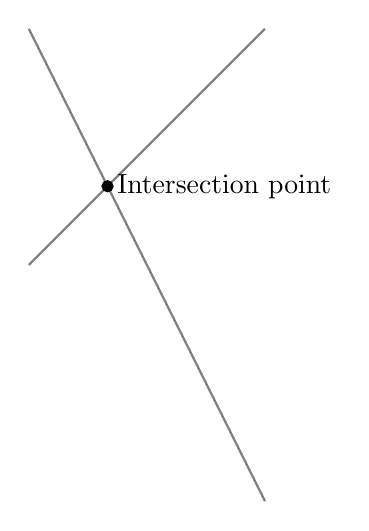
\begin{tikzpicture}
\draw[gray, thick] (-1,2) -- (2,-4);
\draw[gray, thick] (-1,-1) -- (2,2);
\filldraw[black] (0,0) circle (2pt) node[anchor=west]{Intersection point};
\end{tikzpicture}
\caption{Intersecting lines}\label{lines}
\end{figure}
\end{verbatim}
\end{singlespace}

\begin{figure}[!ht]\centering
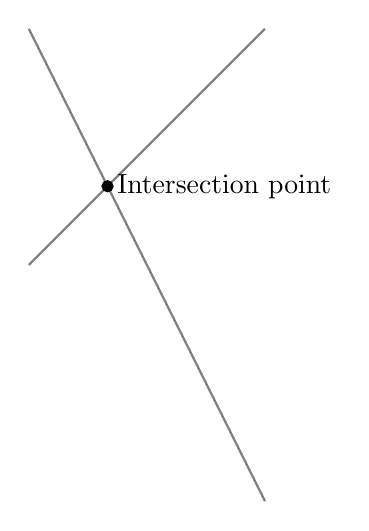
\begin{tikzpicture}
\draw[gray, thick] (-1,2) -- (2,-4);
\draw[gray, thick] (-1,-1) -- (2,2);
\filldraw[black] (0,0) circle (2pt) node[anchor=west]{Intersection point};
\end{tikzpicture}
\caption{Intersecting lines}\label{lines}
\end{figure}

\subsection{Minipages}

You can also create minipages in your documents to accomplish more complicated formatting. For example, you could try the following which produces Figure~\ref{Fig2}.
\begin{singlespace}\small
\begin{verbatim}
\begin{minipage}[t][3 in][t]{1 in}
This is a minipage which is 3 in tall and 1 in wide.
 Top Text Text Text Text.\end{minipage}\hfill
\begin{minipage}[t][3 in][c]{1 in}
This is a minipage which is 3 in tall and 1 in wide.
 Center Text Text Text Text.\end{minipage}\hfill
\begin{minipage}[t][3 in][b]{1 in}
This is a minipage which is 3 in tall and 1 in wide.
 Bottom Text Text Text Text.\end{minipage}
\end{verbatim}
\end{singlespace}

\begin{figure}[!htb]
\begin{minipage}[t][3 in][t]{1 in}
This is a minipage which is 3 in tall and 1 in wide. Top Text Text Text Text.
\end{minipage}
\hfill
\begin{minipage}[t][3 in][c]{1 in} This is a minipage which is 3 in tall and 1 in wide. Center Text Text Text Text.
\end{minipage}
\hfill
\begin{minipage}[t][3 in][b]{1 in}
This is a minipage which is 3 in tall and 1 in wide. Bottom Text Text Text Text.
\end{minipage}
\caption{Minipage example}\label{Fig2}
\end{figure}

In the example above, the syntax \verb|\begin{minipage}[t][3 in][t]{1 in}| follows the convention \linebreak\verb|\begin{minipage}[minipageposition][height][textposition]{width}|\index{minipage}

\subsection[Two pictures in one figure]{How to get more than one picture in the same figure}

You can use minipages to put more than one picture in a figure. Here is an example of how to do this.
\begin{singlespace}\small
\begin{verbatim}
\begin{minipage}[!ht]{6cm}
\woopic{picture1}{.4}
\par
\caption[What goes in the List of Figures]{Left}
\end{minipage}
\hfill
\begin{minipage}[!ht]{6cm}
\woopic{picture2}{.4}
\end{picture}\par
\caption{Right}
\end{minipage}
\end{verbatim}
\end{singlespace}
\begin{figure}[!ht]
\begin{minipage}[!ht]{6cm}
\woopic{picture1}{.4}
\par
\caption[What goes in the List of Figures]{Left}
\end{minipage}
\hfill
\begin{minipage}[!ht]{6cm}
\woopic{picture2}{.4}
\par
\caption{Right}
\end{minipage}
\end{figure}

You can also use the \ip{subfig} package to do this. %changed subfigure to subfig as result of changing to subfig package due to deprecation of subfigure 1-24-2020 - JB

\begin{singlespace}\small
\begin{verbatim}
\begin{figure}[!ht]\centering
\subfloat[What goes in the List][Large conchoid]
{\woopic{picture1}{.4}\label{fig3:left}}
\qquad
\subfloat[What goes in the List][Small conchoid]
{\woopic{picture2}{.4}\label{fig3:right}}
\caption{Two pictures in one figure}\label{fig3}
\end{figure}
\end{verbatim}
\end{singlespace}
\begin{figure}[!ht]\centering
\subfloat[What goes in the List][Large conchoid] %changed subfigure to subfloat as result of changing to subfig package due to deprecation of subfigure 1-24-2020 - JB
{\woopic{picture1}{.4}\label{fig3:left}}
\qquad
\subfloat[What goes in the List][Small conchoid] %changed subfigure to subfloat as result of changing to subfig package due to deprecation of subfigure 1-24-2020 - JB
{\woopic{picture2}{.4}\label{fig3:right}}
\caption{Two pictures in one figure}\label{fig3}
\end{figure}

We should now be able to refer to either Figure~\ref{fig3}~\subref{fig3:left} or Figure~\ref{fig3}~\subref{fig3:right} using the labels we gave to the left and right images.

The reader is referred to Chapters 8, 9, and 16 of \citet{kd03} or to Chapters 6 and 10 of \citet{mgbcr04} for a complete discussion of figures and graphics.

\section{Tables}

Tables are easy to set up. Here is a simple table:
\begin{singlespace}\small
\begin{verbatim}
\begin{table}[!ht]
\begin{center}
\caption{Our first table}
\begin{tabular}{r l}
  $\underline{\textnormal{District}}$ &  
  $\underline{\textnormal{Population}}$\\
   Applewood & 8280 \\
   Boxwood & 4600  \\
   Central & 5220
   \end{tabular}\caption{Our first table}
   \end{center}
\end{table}
\end{verbatim}
\end{singlespace}
\begin{table}[!ht]
\begin{center}
\caption{Our first table}
\begin{tabular}{r l}
  $\underline{\textnormal{District}}$ &
    $\underline{\textnormal{Population}}$\\
   Applewood & 8280 \\
   Boxwood & 4600  \\
   Central & 5220
   \end{tabular}
   \end{center}
\end{table}

In \verb|\begin{tabular}{r l}| the two ``r'' and ``l'' indicate that we have two columns with right and left aligned entries and no lines dividing cells or around the table. I can make the table look more like a spreadsheet by doing:
\begin{singlespace}\small
\begin{verbatim}
\begin{table}[!ht]
\begin{center}
\caption{Our first table again}
\begin{tabular}{|r|l|}
\hline
  {\textnormal{District}} &  
  {\textnormal{Population}}\\ \hline
   Applewood & 8280 \\ \hline
   Boxwood & 4600  \\ \hline
   Central & 5220\\ \hline
   \end{tabular}
   \end{center}
\end{table}
\end{verbatim}
\end{singlespace}
\begin{table}[!ht]
\begin{center}
\caption{Our first table again}
\begin{tabular}{|r|l|}
\hline
  {\textnormal{District}} &  
  {\textnormal{Population}}\\ \hline
   Applewood & 8280 \\ \hline
   Boxwood & 4600  \\ \hline
   Central & 5220\\ \hline
   \end{tabular}
   \end{center}
\end{table}

Here is a more complicated example of a table.
\begin{singlespace}\small
\begin{verbatim}
\begin{table}[!ht]
\caption{Reduction of curvature by each reprojection method\label{tbl:kreduce}}
\centerline{
\begin{tabular}{|l||r|r|r|r|} \hline
\emph{Reprojection} & \multicolumn{3}{|c|}{\emph{Largest
 Reduction of Curvature}}
  & \emph{Average} \\ \cline{2-4}
\emph{Method} & \emph{Original} & \emph{Reprojected} &
 \emph{at} & 
  \emph{Reduction} \\ 
 & \emph{Curvature} & \emph{Curvature} &
  \emph{Rotation} & \emph{of Curvature} \\ 
  \hline \hline
ZEEL & 0.0358 & 0.0245 &
 $\degree{45}$ & 0.0050 \\ \hline
ZEEL ext.\ & 0.0358 & 0.0245 &
 $\degree{45}$ & 0.0059 \\ \hline
Regridding & 0.0428 & 0.0166 &
 $\degree{75}$ & 0.0159 \\ \hline
Block & 0.0358 & 0.0103 &
 $\degree{45}$ & 0.0163 \\ \hline
\end{tabular}}
\end{table}
\end{verbatim}
\end{singlespace}
\begin{table}[!ht]
\caption{Reduction of curvature by each reprojection method\label{tbl:kreduce}}
\centerline{
\begin{tabular}{|l||r|r|r|r|} \hline
\emph{Reprojection} & \multicolumn{3}{|c|}{\emph{Largest Reduction of Curvature}} 
  & \emph{Average} \\ \cline{2-4}
\emph{Method} & \emph{Original} & \emph{Reprojected} & \emph{at} & 
  \emph{Reduction} \\ 
 & \emph{Curvature} & \emph{Curvature} & \emph{Rotation} & \emph{of Curvature} \\ 
  \hline \hline
ZEEL & 0.0358 & 0.0245 & $\degree{45}$ & 0.0050 \\ \hline
ZEEL ext.\ & 0.0358 & 0.0245 & $\degree{45}$ & 0.0059 \\ \hline
Regridding & 0.0428 & 0.0166 & $\degree{75}$ & 0.0159 \\ \hline
Block & 0.0358 & 0.0103 & $\degree{45}$ & 0.0163 \\ \hline
\end{tabular}}
\end{table}

Please refer to Chapter 6 of \citet{kd03} for a complete discussion of tables and tabular environments.
%!TEX root = ../main.tex
\chapter{Working with bibliographies and indicies}\label{bibind}
I would highly recommend that you use Bib\LaTeX{} for your bibliography, and that is what this class uses as of August 2022. Bib\LaTeX{} supports foreign languages and UTF-8 and provides several styles for formatting references (ACS, Chicago, APA, Turabian). For many people it also is easier to customize than Bib\TeX{} with natbib, should you need to customize the formatting of references. Bib\LaTeX{} also can make use of the Biber reference processing application which provides support for foreign languages and more sophisticated sorting options than Bib\TeX{}. You still process a special .bib file. The .bib file is where you enter your bibliographic information. Sample entries look something like
\begin{singlespace}\small
\begin{verbatim}
@article{feu02,
author=		{Thomas Feuerstack},
title=			{Introduction to pdf{\TeX{}}}, 
journal=		{TUGboat}, 
volume=		{23},
pages=		{329--334},
number=		{3/4},
url=			{http://www.tug.org/TUGboat/Articles/tb23-3-4/tb75feu.pdf},
year=			2002}
\end{verbatim}
\end{singlespace}
or
\begin{singlespace}\small
\begin{verbatim}
@book{mgbcr04,
author=		{Frank Mittelbach and Michel Goossens and
Johannes Braams and David Carlisle and Chris Rowley},
title=			{The \LaTeX\ Companion},
publisher=		{Addison Wesley Professional},
edition=		{2nd},
address=		{New York},
year=			2004}
\end{verbatim}
\end{singlespace}

For a Web site I would recommend the following
\begin{singlespace}\small
\begin{verbatim}
@misc{brei04,
author = 		{Jon Breitenbucher},
title = 		{{W}ooster related {L}a{T}e{X} files},
url = 			{https://woolatex.spaces.wooster.edu},
howpublished=	{World Wide Web},
year=			2021,
note = 		{Accessed on 09/27/2021}}
\end{verbatim}
\end{singlespace}

You can make a reference by typing \verb|\citet{mgbcr04}| to produce \citet{mgbcr04}. Other forms for citation include \verb|\citep{mgbcr04}| or  \verb|\citeauthor| \verb|{mgbcr04}| to produce \citep{mgbcr04} or \citeauthor{mgbcr04} respectively. You can consult \citet{kd03} or \citet{mgbcr04} to find out how to format entries in the .bib file and what options each reference type has.\footnote{You could also use footnotes if your department called for that.}

Indicies are also relatively easy to create. If I wanted to have Wooster\index{Wooster} show up in the index, I would enter \verb|Wooster\index{Wooster}| in my source file. I could create a subentry for User Services\index{Wooster!User Services} by entering \verb|User Services|\verb|\index{Wooster!User Services}|. A subsubentry for Help Desk\index{Wooster!User Services!Help Desk} would be entered as \verb|\index{Wooster!User| \verb|Services!Help Desk}|.

To create the index, one needs to make sure to uncomment the \verb|\makeindex| command in the \texttt{main.tex} file. One also needs to uncomment the makeidx entry in the \verb|styles/packages.tex| file and then run the Makeindex program. Consult \citet{kd03} or \citet{mgbcr04} for further information.
\chapter{Challenges and Lessons Learned}\label{text}

\section[What worked well]{What worked well}\label{sec:newsec}
\section[What did not work well ]{What did not work well }\label{sec:newsec}
% %!TEX root = ../main.tex
\chapter{Working with figures and tables}\label{graphics}

\section{Getting a simple figure in the document}
In this chapter we want to talk about including figures and tables in the document. To insert a simple figure, you can enter something like
\begin{singlespace}\small
\begin{verbatim}
\begin{figure}[!ht]
\begin{center}
\woopic{picture3}{.8}
\end{center}
\caption{Our first
 picture}\label{first}
\end{figure}
\end{verbatim}
\end{singlespace}
\vspace{-1.8 in}
\begin{figure}[!ht]
\rightline{
\begin{minipage}{.5\textwidth}
\begin{center}
\woopic{picture3}{.8}
\vspace{-.2 in}
\caption{Our first picture}\label{first}
\end{center}
\end{minipage}
}
\end{figure}

The \verb|!ht| tell \LaTeX{} to try and place the figure here no matter what or at the top of the next page. The \verb|\woopic| command takes the name of the picture as the first argument and the scaling factor as the second argument. The scaling factor must be between zero and one and the figure name must have \emph{no spaces}. Your figures can be in one of four formats: jpg, png, tif, or pdf. Captions are placed below the figure and your label should be placed after the caption.

In the next example we are using the woosterthesis option \verb|picins|\index{woosterthesis options!picins} to typeset a picture inside a paragraph and have the text wrap around the figure. This option loads the \ip{wrapfig} package. One thing to note is that the figures placed in this manner do not float with the other figures and as such numbering could get out of sequence. Keep an eye out for such behavior.  This technique should be used sparingly in your thesis.

\begin{singlespace}\small
\begin{verbatim}
\newcommand{\sample}{Some text that is reused over and over
 again in the example. }
\begin{wrapfigure}{r}{2.2in}
\woopic{picture2}{.4}
\caption{Conchoid.}
\end{wrapfigure}
\sample\sample\sample\sample
\end{verbatim}
\end{singlespace}

\newcommand{\sample}{Some text that is reused over and over again in the example. }
\begin{wrapfigure}{r}{2.2in}
\woopic{picture2}{.4}
\caption{Conchoid.}
\end{wrapfigure}
\sample\sample\sample\sample\sample\sample\sample\sample\sample

\subsection{Drawing figures in \LaTeX{}}

It is also possible to use the \ip{Ti\emph{k}Z} package to draw figures like Figures \ref{tree} or \ref{lines} in your document. Ti\emph{k}Z/PGF are a pair of languages that allow users to create vector graphics as part of their \LaTeX{} document using commands that are \TeX{} macros. It is possible to create extremely complex scalable graphics using Ti\emph{k}Z, see the \href{https://en.wikipedia.org/wiki/PGF/TikZ}{Ti\emph{k}Z wikipedia entry} for some examples.

\begin{singlespace}\small
\begin{verbatim}
\begin{figure}[!ht]\centering
\begin{tikzpicture}[
roundnode/.style={circle, draw=green!60, fill=green!5, very thick, minimum size=7mm},
squarednode/.style={rectangle, draw=red!60, fill=red!5, very thick, minimum size=5mm},
]
%Nodes
\node[squarednode]      (maintopic)                              {2};
\node[roundnode]        (uppercircle)       [above=of maintopic] {1};
\node[squarednode]      (rightsquare)       [right=of maintopic] {3};
\node[roundnode]        (lowercircle)       [below=of maintopic] {4};
%Lines
\draw[->] (uppercircle.south) -- (maintopic.north);
\draw[->] (maintopic.east) -- (rightsquare.west);
\draw[->] (rightsquare.south) .. controls +(down:7mm) and +(right:7mm) .. (lowercircle.east);
\end{tikzpicture}
\caption{Tree diagram}\label{tree}
\end{figure}
\end{verbatim}
\end{singlespace}

\begin{figure}[!ht]\centering
\begin{tikzpicture}[
roundnode/.style={circle, draw=green!60, fill=green!5, very thick, minimum size=7mm},
squarednode/.style={rectangle, draw=red!60, fill=red!5, very thick, minimum size=5mm},
]
%Nodes
\node[squarednode]      (maintopic)                              {2};
\node[roundnode]        (uppercircle)       [above=of maintopic] {1};
\node[squarednode]      (rightsquare)       [right=of maintopic] {3};
\node[roundnode]        (lowercircle)       [below=of maintopic] {4};

%Lines
\draw[->] (uppercircle.south) -- (maintopic.north);
\draw[->] (maintopic.east) -- (rightsquare.west);
\draw[->] (rightsquare.south) .. controls +(down:7mm) and +(right:7mm) .. (lowercircle.east);
\end{tikzpicture}
\caption{Tree diagram}\label{tree}
\end{figure}

\begin{singlespace}\small
\begin{verbatim}
\begin{figure}[!ht]\centering
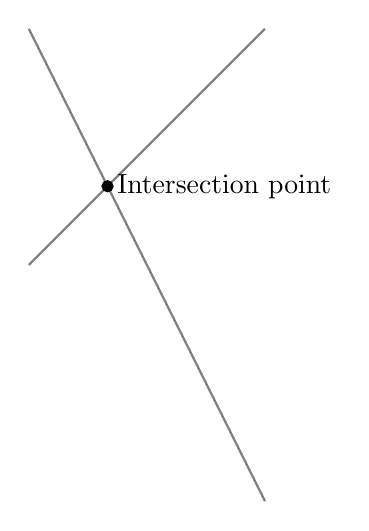
\begin{tikzpicture}
\draw[gray, thick] (-1,2) -- (2,-4);
\draw[gray, thick] (-1,-1) -- (2,2);
\filldraw[black] (0,0) circle (2pt) node[anchor=west]{Intersection point};
\end{tikzpicture}
\caption{Intersecting lines}\label{lines}
\end{figure}
\end{verbatim}
\end{singlespace}

\begin{figure}[!ht]\centering
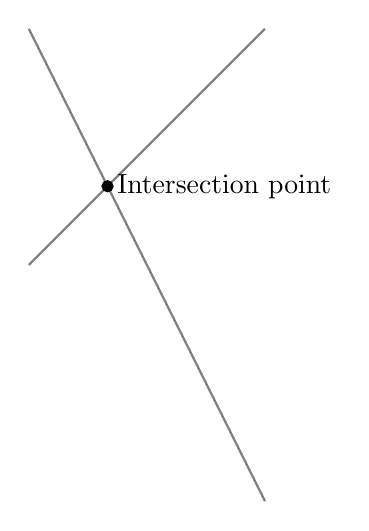
\begin{tikzpicture}
\draw[gray, thick] (-1,2) -- (2,-4);
\draw[gray, thick] (-1,-1) -- (2,2);
\filldraw[black] (0,0) circle (2pt) node[anchor=west]{Intersection point};
\end{tikzpicture}
\caption{Intersecting lines}\label{lines}
\end{figure}

\subsection{Minipages}

You can also create minipages in your documents to accomplish more complicated formatting. For example, you could try the following which produces Figure~\ref{Fig2}.
\begin{singlespace}\small
\begin{verbatim}
\begin{minipage}[t][3 in][t]{1 in}
This is a minipage which is 3 in tall and 1 in wide.
 Top Text Text Text Text.\end{minipage}\hfill
\begin{minipage}[t][3 in][c]{1 in}
This is a minipage which is 3 in tall and 1 in wide.
 Center Text Text Text Text.\end{minipage}\hfill
\begin{minipage}[t][3 in][b]{1 in}
This is a minipage which is 3 in tall and 1 in wide.
 Bottom Text Text Text Text.\end{minipage}
\end{verbatim}
\end{singlespace}

\begin{figure}[!htb]
\begin{minipage}[t][3 in][t]{1 in}
This is a minipage which is 3 in tall and 1 in wide. Top Text Text Text Text.
\end{minipage}
\hfill
\begin{minipage}[t][3 in][c]{1 in} This is a minipage which is 3 in tall and 1 in wide. Center Text Text Text Text.
\end{minipage}
\hfill
\begin{minipage}[t][3 in][b]{1 in}
This is a minipage which is 3 in tall and 1 in wide. Bottom Text Text Text Text.
\end{minipage}
\caption{Minipage example}\label{Fig2}
\end{figure}

In the example above, the syntax \verb|\begin{minipage}[t][3 in][t]{1 in}| follows the convention \linebreak\verb|\begin{minipage}[minipageposition][height][textposition]{width}|\index{minipage}

\subsection[Two pictures in one figure]{How to get more than one picture in the same figure}

You can use minipages to put more than one picture in a figure. Here is an example of how to do this.
\begin{singlespace}\small
\begin{verbatim}
\begin{minipage}[!ht]{6cm}
\woopic{picture1}{.4}
\par
\caption[What goes in the List of Figures]{Left}
\end{minipage}
\hfill
\begin{minipage}[!ht]{6cm}
\woopic{picture2}{.4}
\end{picture}\par
\caption{Right}
\end{minipage}
\end{verbatim}
\end{singlespace}
\begin{figure}[!ht]
\begin{minipage}[!ht]{6cm}
\woopic{picture1}{.4}
\par
\caption[What goes in the List of Figures]{Left}
\end{minipage}
\hfill
\begin{minipage}[!ht]{6cm}
\woopic{picture2}{.4}
\par
\caption{Right}
\end{minipage}
\end{figure}

You can also use the \ip{subfig} package to do this. %changed subfigure to subfig as result of changing to subfig package due to deprecation of subfigure 1-24-2020 - JB

\begin{singlespace}\small
\begin{verbatim}
\begin{figure}[!ht]\centering
\subfloat[What goes in the List][Large conchoid]
{\woopic{picture1}{.4}\label{fig3:left}}
\qquad
\subfloat[What goes in the List][Small conchoid]
{\woopic{picture2}{.4}\label{fig3:right}}
\caption{Two pictures in one figure}\label{fig3}
\end{figure}
\end{verbatim}
\end{singlespace}
\begin{figure}[!ht]\centering
\subfloat[What goes in the List][Large conchoid] %changed subfigure to subfloat as result of changing to subfig package due to deprecation of subfigure 1-24-2020 - JB
{\woopic{picture1}{.4}\label{fig3:left}}
\qquad
\subfloat[What goes in the List][Small conchoid] %changed subfigure to subfloat as result of changing to subfig package due to deprecation of subfigure 1-24-2020 - JB
{\woopic{picture2}{.4}\label{fig3:right}}
\caption{Two pictures in one figure}\label{fig3}
\end{figure}

We should now be able to refer to either Figure~\ref{fig3}~\subref{fig3:left} or Figure~\ref{fig3}~\subref{fig3:right} using the labels we gave to the left and right images.

The reader is referred to Chapters 8, 9, and 16 of \citet{kd03} or to Chapters 6 and 10 of \citet{mgbcr04} for a complete discussion of figures and graphics.

\section{Tables}

Tables are easy to set up. Here is a simple table:
\begin{singlespace}\small
\begin{verbatim}
\begin{table}[!ht]
\begin{center}
\caption{Our first table}
\begin{tabular}{r l}
  $\underline{\textnormal{District}}$ &  
  $\underline{\textnormal{Population}}$\\
   Applewood & 8280 \\
   Boxwood & 4600  \\
   Central & 5220
   \end{tabular}\caption{Our first table}
   \end{center}
\end{table}
\end{verbatim}
\end{singlespace}
\begin{table}[!ht]
\begin{center}
\caption{Our first table}
\begin{tabular}{r l}
  $\underline{\textnormal{District}}$ &
    $\underline{\textnormal{Population}}$\\
   Applewood & 8280 \\
   Boxwood & 4600  \\
   Central & 5220
   \end{tabular}
   \end{center}
\end{table}

In \verb|\begin{tabular}{r l}| the two ``r'' and ``l'' indicate that we have two columns with right and left aligned entries and no lines dividing cells or around the table. I can make the table look more like a spreadsheet by doing:
\begin{singlespace}\small
\begin{verbatim}
\begin{table}[!ht]
\begin{center}
\caption{Our first table again}
\begin{tabular}{|r|l|}
\hline
  {\textnormal{District}} &  
  {\textnormal{Population}}\\ \hline
   Applewood & 8280 \\ \hline
   Boxwood & 4600  \\ \hline
   Central & 5220\\ \hline
   \end{tabular}
   \end{center}
\end{table}
\end{verbatim}
\end{singlespace}
\begin{table}[!ht]
\begin{center}
\caption{Our first table again}
\begin{tabular}{|r|l|}
\hline
  {\textnormal{District}} &  
  {\textnormal{Population}}\\ \hline
   Applewood & 8280 \\ \hline
   Boxwood & 4600  \\ \hline
   Central & 5220\\ \hline
   \end{tabular}
   \end{center}
\end{table}

Here is a more complicated example of a table.
\begin{singlespace}\small
\begin{verbatim}
\begin{table}[!ht]
\caption{Reduction of curvature by each reprojection method\label{tbl:kreduce}}
\centerline{
\begin{tabular}{|l||r|r|r|r|} \hline
\emph{Reprojection} & \multicolumn{3}{|c|}{\emph{Largest
 Reduction of Curvature}}
  & \emph{Average} \\ \cline{2-4}
\emph{Method} & \emph{Original} & \emph{Reprojected} &
 \emph{at} & 
  \emph{Reduction} \\ 
 & \emph{Curvature} & \emph{Curvature} &
  \emph{Rotation} & \emph{of Curvature} \\ 
  \hline \hline
ZEEL & 0.0358 & 0.0245 &
 $\degree{45}$ & 0.0050 \\ \hline
ZEEL ext.\ & 0.0358 & 0.0245 &
 $\degree{45}$ & 0.0059 \\ \hline
Regridding & 0.0428 & 0.0166 &
 $\degree{75}$ & 0.0159 \\ \hline
Block & 0.0358 & 0.0103 &
 $\degree{45}$ & 0.0163 \\ \hline
\end{tabular}}
\end{table}
\end{verbatim}
\end{singlespace}
\begin{table}[!ht]
\caption{Reduction of curvature by each reprojection method\label{tbl:kreduce}}
\centerline{
\begin{tabular}{|l||r|r|r|r|} \hline
\emph{Reprojection} & \multicolumn{3}{|c|}{\emph{Largest Reduction of Curvature}} 
  & \emph{Average} \\ \cline{2-4}
\emph{Method} & \emph{Original} & \emph{Reprojected} & \emph{at} & 
  \emph{Reduction} \\ 
 & \emph{Curvature} & \emph{Curvature} & \emph{Rotation} & \emph{of Curvature} \\ 
  \hline \hline
ZEEL & 0.0358 & 0.0245 & $\degree{45}$ & 0.0050 \\ \hline
ZEEL ext.\ & 0.0358 & 0.0245 & $\degree{45}$ & 0.0059 \\ \hline
Regridding & 0.0428 & 0.0166 & $\degree{75}$ & 0.0159 \\ \hline
Block & 0.0358 & 0.0103 & $\degree{45}$ & 0.0163 \\ \hline
\end{tabular}}
\end{table}

Please refer to Chapter 6 of \citet{kd03} for a complete discussion of tables and tabular environments.
% %!TEX root = ../main.tex
\chapter{Working with bibliographies and indicies}\label{bibind}
I would highly recommend that you use Bib\LaTeX{} for your bibliography, and that is what this class uses as of August 2022. Bib\LaTeX{} supports foreign languages and UTF-8 and provides several styles for formatting references (ACS, Chicago, APA, Turabian). For many people it also is easier to customize than Bib\TeX{} with natbib, should you need to customize the formatting of references. Bib\LaTeX{} also can make use of the Biber reference processing application which provides support for foreign languages and more sophisticated sorting options than Bib\TeX{}. You still process a special .bib file. The .bib file is where you enter your bibliographic information. Sample entries look something like
\begin{singlespace}\small
\begin{verbatim}
@article{feu02,
author=		{Thomas Feuerstack},
title=			{Introduction to pdf{\TeX{}}}, 
journal=		{TUGboat}, 
volume=		{23},
pages=		{329--334},
number=		{3/4},
url=			{http://www.tug.org/TUGboat/Articles/tb23-3-4/tb75feu.pdf},
year=			2002}
\end{verbatim}
\end{singlespace}
or
\begin{singlespace}\small
\begin{verbatim}
@book{mgbcr04,
author=		{Frank Mittelbach and Michel Goossens and
Johannes Braams and David Carlisle and Chris Rowley},
title=			{The \LaTeX\ Companion},
publisher=		{Addison Wesley Professional},
edition=		{2nd},
address=		{New York},
year=			2004}
\end{verbatim}
\end{singlespace}

For a Web site I would recommend the following
\begin{singlespace}\small
\begin{verbatim}
@misc{brei04,
author = 		{Jon Breitenbucher},
title = 		{{W}ooster related {L}a{T}e{X} files},
url = 			{https://woolatex.spaces.wooster.edu},
howpublished=	{World Wide Web},
year=			2021,
note = 		{Accessed on 09/27/2021}}
\end{verbatim}
\end{singlespace}

You can make a reference by typing \verb|\citet{mgbcr04}| to produce \citet{mgbcr04}. Other forms for citation include \verb|\citep{mgbcr04}| or  \verb|\citeauthor| \verb|{mgbcr04}| to produce \citep{mgbcr04} or \citeauthor{mgbcr04} respectively. You can consult \citet{kd03} or \citet{mgbcr04} to find out how to format entries in the .bib file and what options each reference type has.\footnote{You could also use footnotes if your department called for that.}

Indicies are also relatively easy to create. If I wanted to have Wooster\index{Wooster} show up in the index, I would enter \verb|Wooster\index{Wooster}| in my source file. I could create a subentry for User Services\index{Wooster!User Services} by entering \verb|User Services|\verb|\index{Wooster!User Services}|. A subsubentry for Help Desk\index{Wooster!User Services!Help Desk} would be entered as \verb|\index{Wooster!User| \verb|Services!Help Desk}|.

To create the index, one needs to make sure to uncomment the \verb|\makeindex| command in the \texttt{main.tex} file. One also needs to uncomment the makeidx entry in the \verb|styles/packages.tex| file and then run the Makeindex program. Consult \citet{kd03} or \citet{mgbcr04} for further information.
%\chapter{Challenges and Lessons Learned}\label{text}

\section[What worked well]{What worked well}\label{sec:newsec}
\section[What did not work well ]{What did not work well }\label{sec:newsec}
%\input{chapters/chapter5}
%\input{chapters/chapter6}
%\input{chapters/chapter7}
%\input{conclusion}

%%%%%%%%%%%%%%%%%%%%%%%%%%%%%%%%%%%%%%%%%%%%%%%%%%%%%%%
%
%  This section starts the back matter. The back matter includes appendices, indicies, and the
%  bibliography
%
%%%%%%%%%%%%%%%%%%%%%%%%%%%%%%%%%%%%%%%%%%%%%%%%%%%%%%%

\backmatter

% \input{appendices/math}
% \input{appendices/java}
% \input{appendices/cpp}
% \input{appendices/options}
% \input{appendices/afterword}

%%%%%%%%%%%%%%%%%%%%%%%%%%%%%%%%%%%%%%%%%%%%%%%%%%%%%%%
%
%  We used BibLaTeX and Biber to generate a Bibliography.
%
%%%%%%%%%%%%%%%%%%%%%%%%%%%%%%%%%%%%%%%%%%%%%%%%%%%%%%%

\nocite{*} % This command forces all the bibliography references to be printed -- not just 
              % those that were explicitly cited in the text.  If you comment this out, the bibliography
              % will only include cited references.
\printbibliography[title=References,heading=bibintoc]% load our Bibliography file

%%%%%%%%%%%%%%%%%%%%%%%%%%%%%%%%%%%%%%%%%%%%%%%%%%%%%%%
%
%                                                                Index
%
%  Uncomment the lines below to include an index. To get an index you must put 
%  \index{index text} after any words that you want to appear in the index.
%  Subentries are entered as \index{index text!subentry text}. You must also run the

%  makeindex program to generate the index files that LaTeX uses. The PCs are set to run
%  makeindex automatically.
%
%%%%%%%%%%%%%%%%%%%%%%%%%%%%%%%%%%%%%%%%%%%%%%%%%%%%%%%

\ifthenelse{\boolean{index}}{
\cleardoublepage
\phantomsection
\addcontentsline{toc}{chapter}{Index}
\printindex}{}

%%%%%%%%%%%%%%%%%%%%%%%%%%%%%%%%%%%%%%%%%%%%%%%%%%%%%%%
%
%                                                                Colophon
%
%  A Colophon is a section of a printed document that acknowledges the designers and printers of the work.
% The colophon also includes information about the fonts and paper used in the printing. It is not required 
% for your IS and can be commented out.
%
%%%%%%%%%%%%%%%%%%%%%%%%%%%%%%%%%%%%%%%%%%%%%%%%%%%%%%%

\ifthenelse{\boolean{colophon}}{
\begin{colophon}
This Independent Study was designed by Dr. Jon Breitenbucher.\newline
It was edited and set into type in Wooster, Ohio,\newline
using the \ifthenelse{\boolean{xetex}}{\XeTeX\ typesetting system designed by Jonathan Kew}{\LaTeX\ typesetting system designed by Leslie Lamport}\newline
and based on the original \TeX\ system of Donald Knuth.\newline

The text face is Palatino, designed by Hermann Zapf in 1948,\newline
and initially released in 1949 by the Stempel foundry and later\newline
by other companies, most notably the Mergenthaler Linotype\newline
Company. Palatino is optimised for legitibility with open counters,\newline
balanced proportions, moderate stroke contrast and flared serifs.
\end{colophon}}{}
\clearpage\thispagestyle{empty}\null\clearpage
\end{document}